\documentclass{article}
\usepackage[utf8]{inputenc}
\usepackage[margin = 0.78in]{geometry}
\usepackage{amsmath, amssymb}
\usepackage{graphicx}
\usepackage{caption}
\usepackage{subcaption}
\usepackage{cite}
\usepackage{hyperref}   % use this instead of \usepackage{url}
\usepackage{float}
\usepackage{outlines}
\usepackage{booktabs}
\usepackage{tabularx}
\usepackage{readarray} % For parsing csv into an array before placing in matrix
\usepackage{pgf}
\usepackage{pythonhighlight}
\usepackage{numprint}
\usepackage{color, colortbl}
% Copied packages directly from a previous path planning analysis assignment - may need updating

\pgfkeys{/pgf/number format/.cd,precision=6,sci,sci e} % generic={exponent={\times 10^{#1}}}}
\newcommand\convert[1]{\pgfmathprintnumber{#1}}
\npdecimalsign{.}
\nprounddigits{7}
\definecolor{yellow}{rgb}{1, 1, 0}
\setcounter{MaxMatrixCols}{15}  % expands maximum \bmatrix size to 15

\title{RBE 577 - Nonlinear Navigation Filters Assignment}
\author{Everett Wenzlaff (ecwenzlaff@wpi.edu)}
\date{Due: May 7, 2025}

\begin{document}
\maketitle

\section{Introduction}
The purpose of this assignment is to implement a control allocator based on the findings from R. Skulstad et. al.'s ``Constrained control allocation for dynamic ship positioning using deep neural network''\cite{paper}. The primary objective of the paper involved designing a deep neural network (DNN) to perform optimal control allocation for the torque commands received by a ship's motion controller. While we don't have access to all of the data or parameters used for testing the specific implementation, the paper described the basic architecture and sampling methods used to train their DNN. This high level description for architecture and sampling will be used as the starting point for this assignment.

\section{Methodology}
The basic architecture for the paper's DNN took the form of a symmetrical autoencoder. The autoencoder consisted of a symmetrical 3 layer encoder, and a 3 layer decoder, which each contained two layers of Long Short-Term Memory (LSTM) nodes. While autoencoders are typically used to reduce the dimensionality of the latent space compared to the inputs, the autoencoder from the paper converted 3 ``generalized" torques, $\left[\tau_{surge}, \tau_{sway}, \tau_{yaw}\right]^{T}$, into separate forces and angle components within its latent space based on the configuration of the ship (see Figure \ref{fig:ship} below). The forces, $\left[F_1, F_2, F_3\right]$, and angles, $\left[\alpha_2, \alpha_3\right]$, in the latent space represent the control allocator commands, $\hat{u}$, for the ship's thrusters.

\begin{figure}[H]
    \centering
    \begin{subfigure}{0.55\textwidth}
        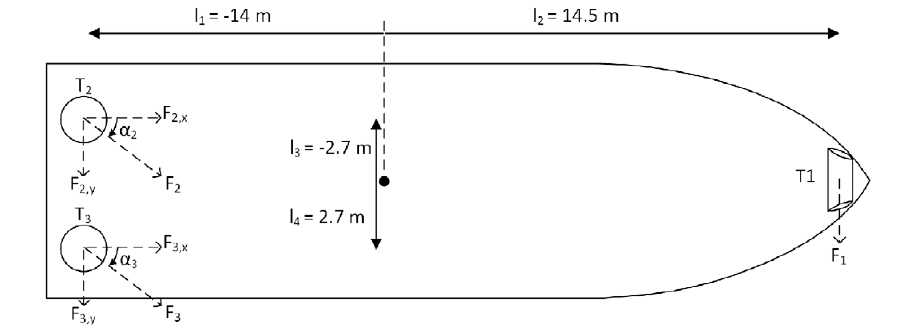
\includegraphics[width=\textwidth]{./ship.png}
        \caption{}
    \end{subfigure} 
    \begin{subfigure}{0.6\textwidth}
        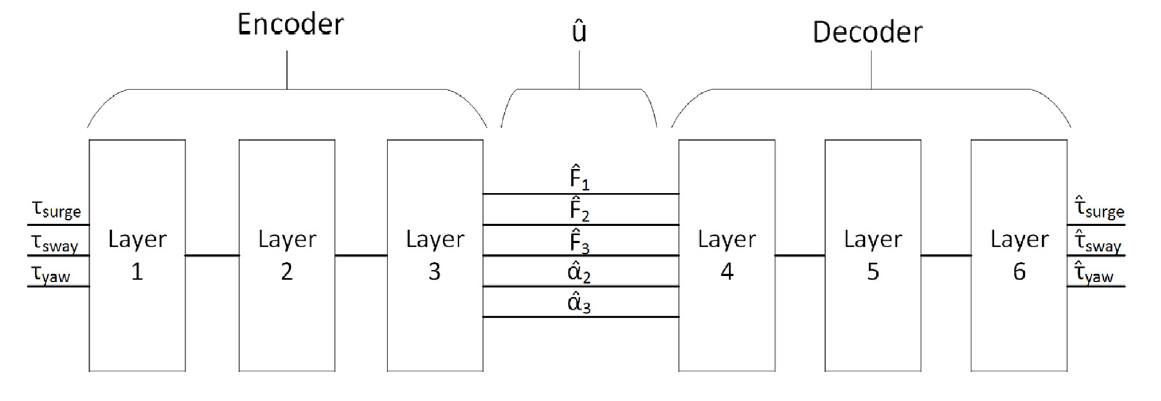
\includegraphics[width=\textwidth]{./autoencoder.png}
        \caption{}
    \end{subfigure}
    \caption{The autoencoder in (b) converts the generalized torques requested from the ship's motion controller to direct commands for the ship's thrusters, $T1$, $T2$, and $T3$ in (b). Since $T1$ is a non-rotatable thruster, only thrusters $T2$ and $T3$ can receive angle commands ($\alpha_2$, and $\alpha_3$).}
    \label{fig:ship}
\end{figure}

While the paper described testing the autoencoder using outputs from a high fidelity ship simulator (which cannot be reproduced for this assignment), the autoencoder was trained using randomly generated data. More specifically, the paper described generating data with a randomly initialized random walk for each of the thruster command components, and provided the associated upper and lower bounds. These randomly generated thruster commands were then converted into generalized torque inputs via the following transformation:
\begin{gather*}
    \begin{bmatrix}
        \tau_{surge} \\
        \tau_{sway} \\
        \tau_{yaw}
    \end{bmatrix}
    =
    \begin{bmatrix}
        0 & \cos \left(\alpha_2\right) & \cos \left(\alpha_3\right) \\ 
        1 & \sin \left(\alpha_2\right) & \sin \left(\alpha_3\right) \\
        l_2 & l_1 \sin \left(\alpha_2\right) - l_3 \cos \left(\alpha_2\right) & l_1 \sin \left(\alpha_3\right) - l_4\cos\left(\alpha_3\right)
    \end{bmatrix}
    \dot{}
    \begin{bmatrix}
        F_1 \\
        F_2 \\
        F_3 
    \end{bmatrix}
\end{gather*}
And as part of the autoencoder training, the paper also described a series of different loss functions that were used to drive the output behavior. The separate loss functions were then scaled (according to importance and magnitude) and combined to form a single loss value to facilitate optimization. The individual loss functions can be described as follows:
\begin{itemize}
    \item $L0$ computed the mean square error (MSE) between the generalized input torques and the torques resulting from directly transforming the encoder's commanded outputs in order to align the inputs with the encoder outputs.
    \item $L1$ computed the MSE between the generalized input torques and the torques output from the decoder in order to align the inputs with the decoder outputs.
    \item $L2$ returned values for individual encoder components that exceeded respective predefined limits in order to minimize the magnitude of the encoder commands.
    \item $L3$ returned values which penalized large rate changes in the encoder commands.
    \item $L4$ computed an estimate of the power output from the encoder commands in an attempt to minimize power consumption.
    \item $L5$ returned values based on the encoder command angle outputs in order to minimize the time that the thrusters are commanded to operate within ``inefficient azimuth sectors''.
\end{itemize}

So in the spirit of using the paper as a starting point, I started implementing the random walk and autoencoder architecture in Python. 

\section{Results}

\section{Discussion}

\begin{thebibliography}{99}
    \bibitem{paper} Skulstad, R. (2023) (PDF) constrained control allocation for dynamic ship positioning using Deep Neural Network, ResearchGate. Available at: \url{https://www.researchgate.net/publication/369978600\_Constrained\_Control\_Allocation\_for\_Dynamic\_Ship\_Positioning\_using\_Deep\_Neural\_Network}. 
\end{thebibliography}
\end{document}